\setcounter{chapter}{6}

\addcontentsline{toc}{section}{Homework 6}
\section*{Homework 6}

\begin{enumerate}
    \item \textit{Either give an example, or show that no such example exists.}
    
    A bounded function $h$ on $[0,3]$ such that for every partition $P$ of $[0,3]$, $U(h,P) = 5$ and $L(h,P) = 1$

    \begin{proof}[Solution]
        Consider: $h(x) = \begin{cases}
        \frac{5}{3}, & x \in \mathbb{Q} \\
        \frac{1}{3}, & x \notin \mathbb{Q}
        \end{cases}$

        \begin{center}
        \begin{tikzpicture}
            \begin{axis}[
                axis lines=middle,
                xlabel={$x$},
                ylabel={$y$},
                xmin=-0.5, xmax=3.5,
                ymin=0, ymax=2,
                xtick={0,1,2,3},
                ytick={1/3,5/3},
                yticklabels={$\frac{1}{3}$,$\frac{5}{3}$},
                width=10cm,
                height=6cm
            ]
            \addplot[domain=0:3, samples=2, very thick, blue] {1/3};
            \addplot[domain=0:3, samples=2, thin, red] {5/3};
            \end{axis}
        \end{tikzpicture}
        \end{center}

        $h$ is bounded by TREE(3).
        For all partitions, the upper sum is $5$ and the lower sum is $1$.
    \end{proof}

    A function $g$ on $[0,1]$ and partitions $P$ and $Q$ of $[0,1]$ where $U(g,P) = L(g,P)$ but $U(g,Q) \neq L(g,Q)$.
    
    \begin{proof}[Solution]
        Consider the function $g(x) = x$ on $[0,1]$.

            Let $P = \{0, 1\}$ and $Q = \{0, \frac{1}{2}, 1\}$.

            For partition $P$, the upper sum $U(g,P) = L(g,P) = \frac{1}{2}$.

            For partition $Q$, the upper sum $U(g,Q) \neq L(g,Q)$.

            \begin{center}
            \begin{tabular}{cc}
            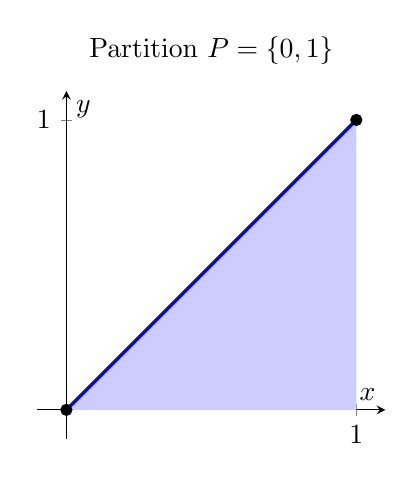
\begin{tikzpicture}
                \begin{axis}[
                axis lines=middle,
                xlabel={$x$},
                ylabel={$y$},
                xmin=-0.1, xmax=1.1,
                ymin=-0.1, ymax=1.1,
                xtick={0,1},
                ytick={0,1},
                width=6cm,
                height=6cm,
                title={Partition $P = \{0, 1\}$}
                ]
                % Shaded area (upper and lower sum coincide for partition P)
                \addplot[fill=blue!20, draw=none, domain=0:1] {x} \closedcycle;
                
                % The function g(x) = x
                \addplot[domain=0:1, samples=2, very thick, blue] {x};
                
                % Mark partition points
                \addplot[only marks, mark=*, mark size=2pt] coordinates {(0,0) (1,1)};
                \end{axis}
            \end{tikzpicture}
            &
            \begin{tikzpicture}
                \begin{axis}[
                axis lines=middle,
                xlabel={$x$},
                ylabel={$y$},
                xmin=-0.1, xmax=1.1,
                ymin=-0.1, ymax=1.1,
                xtick={0,0.5,1},
                ytick={0,0.5,1},
                xticklabels={$0$,$\frac{1}{2}$,$1$},
                yticklabels={$0$,$\frac{1}{2}$,$1$},
                width=6cm,
                height=6cm,
                title={Partition $Q = \{0, \frac{1}{2}, 1\}$}
                ]
                % Lower sum rectangles (northeast lines)
                \addplot[fill=blue!20, pattern=north east lines, pattern color=blue, draw=black] 
                coordinates {(0,0) (0.5,0) (0.5,0) (0,0)} \closedcycle;
                \addplot[fill=blue!20, pattern=north east lines, pattern color=blue, draw=black] 
                coordinates {(0.5,0) (1,0) (1,0.5) (0.5,0.5) (0.5,0)} \closedcycle;
                
                % Upper sum rectangles (northwest lines)
                \addplot[fill=red!20, pattern=north west lines, pattern color=red, draw=black] 
                coordinates {(0,0) (0.5,0) (0.5,0.5) (0,0.5) (0,0)} \closedcycle;
                \addplot[fill=red!20, pattern=north west lines, pattern color=red, draw=black] 
                coordinates {(0.5,0.5) (1,0.5) (1,1) (0.5,1) (0.5,0.5)} \closedcycle;
                
                % The function g(x) = x
                \addplot[domain=0:1, samples=2, very thick, blue] {x};
                
                % Mark partition points
                \addplot[only marks, mark=*, mark size=2pt] coordinates {(0,0) (0.5,0.5) (1,1)};
                \end{axis}
            \end{tikzpicture}
            \end{tabular}
            \end{center}
    \end{proof}

    \pagebreak

    \item \textit{True or False? Give a proof or a counter-example.}
    
    \rule{1cm}{0.15mm} If $g$ is integrable on $[0,1]$, then so is $g(x^n)$, for all $n \in \mathbb{N}$.
    \begin{proof}[Solution]
        True.

        Assume $g$ is integrable on $[0,1]$.
        Then, $\int_{0}^{1} g(x)dx = U(g) = L(g)$.

        For the case where $n = 1$, we have $g(x^1) = g(x)$, which is integrable.

        Now, assume $g(x^k)$ is integrable for some $k \in \mathbb{N}$.
        
        Need to show: $g(x^{k+1})$ is integrable.

        Since $g(x^k)$ is integrable, for every $\epsilon > 0$, there exists a partition $P$ of $[0,1]$ such that $U(g(x^k), P) - L(g(x^k), P) < \epsilon$.
        
        Consider the same partition $P$ for $g(x^{k+1})$.
        
        Note that $x^{k+1} = x \cdot x^k$.
        
        Since $x \in [0,1]$, we have $x^{k+1} \leq x^k$ for all $x \in [0,1]$.

        So, $U(g(x^{k+1}), P) \leq U(g(x^k), P)$ and $L(g(x^{k+1}), P) \leq L(g(x^k), P)$.
        
        Therefore, $U(g(x^{k+1}), P) - L(g(x^{k+1}), P) \leq U(g(x^k), P) - L(g(x^k), P) < \epsilon$.
        
        By induction, $g(x^n)$ is integrable for all $n \in \mathbb{N}$.
    \end{proof}

    \begin{note}
        The above problem makes intuitive sense, it really feels like it just \textit{should} be true.

        All we're doing is shifting the $x$'s (shrinking them, since we're in $[0,1]$), and adjusting the functional value accordingly.

        And since $g$ is integrable, we shouldn't have any issue just moving the $x$'s and functional values around, the result should still be integrable.

        And luckily for us, it is.
    \end{note}

    \rule{1cm}{0.15mm} If $|f|$ is integrable on $[a,b]$, then so is $f$.
    \begin{proof}[Solution]
        False.

        Consider this modified Direchlet function on $[0,1]$:
        \[f(x) = \begin{cases}
        1, & x \in \mathbb{Q} \\
        -1, & x \notin \mathbb{Q}
        \end{cases}\]
        
        So, $|f(x)| = 1$ for all $x \in [0,1]$.

        Thus, $|f|$ is integrable on $[0,1]$.

        But, the Direchlet function is not integrable.
    \end{proof}

    \rule{1cm}{0.15mm} If $f$ and $|f|$ are integrable on $[a,b]$, then $|\int_{a}^{b}f| \leq \int_{a}^{b}|f|$.
    \begin{proof}[Solution]
        True.

        Since $f$ is integrable on $[a,b]$, we have:$\int_{a}^{b}f = L(f) = U(f) \ \ (1) $.

        Since $|f|$ is integrable on $[a,b]$, we have: $\int_{a}^{b}|f| = L(|f|) = U(|f|) \ \ (2)$.

        Notice: $f \leq |f|$ for all $x \in [a,b]$.

        By $(1)$: $|\int_{a}^{b}f| = |U(f)| = | \inf\{U(f,P) : P \text{ is a partition of } [a,b]\} |$.

        By $(2)$: $\int_{a}^{b}|f| = U(|f|) = \inf\{U(|f|,P) : P \text{ is a partition of } [a,b]\}$.

        Each $U(f,P) \leq U(|f|,P) \Rightarrow U(f) \leq U(|f|)$
        $\Leftrightarrow |U(f)| \leq U(|f|)$
        Since $|f| \geq 0$, so:

        $|U(f)| \leq U(|f|)$,

        Thus:

        \[| \int_{a}^{b}f | \leq \int_{a}^{b}|f| \]
    \end{proof}
    \pagebreak
    \item For every $n\ \in \ \mathbb{N}$ and for $x \in \mathbb{R}$, define $g_n(x) = \begin{cases} \frac{1}{n}, & \text{for } -n \leq x \leq n \\ 0, & \text{otherwise} \end{cases}$.
    
    Evaluate the integral $I_n = \int_{-100}^{100} g_n$.
    \begin{note}

    Before we tackle this, we kinda need to do a bunch of work.

    We need to figure out what this function looks like, and what it's integrals will look like.

    Let's start figuring out what some of the $g_n$'s look like, both graphically and functionally.

    Then, we can determine their "areas under the curve", which will help us figure out what we need to do to compute this integral.
    \end{note}
    

    \begin{proof}[Solution]
        First, let's look at a generic graph of $g_n$.

            \begin{center}
            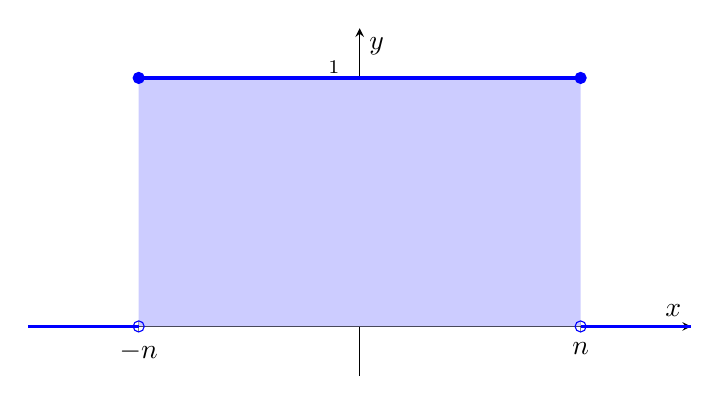
\begin{tikzpicture}
                \begin{axis}[
                axis lines=middle,
                xlabel={$x$},
                ylabel={$y$},
                xmin=-1.5, xmax=1.5,
                ymin=-0.2, ymax=1.2,
                xtick={-1,0,1},
                xticklabels={$-n$,$0$,$n$},
                ytick={0,1},
                yticklabels={$0$,$\frac{1}{n}$},
                width=10cm,
                height=6cm
                ]
                % Shaded area under the curve
                \addplot[fill=blue!20, draw=none] coordinates {(-1,0) (-1,1) (1,1) (1,0)} \closedcycle;
                
                % The function g_n(x)
                \addplot[domain=-1:1, samples=2, very thick, blue] {1};
                \addplot[domain=-1.5:-1, samples=2, very thick, blue] {0};
                \addplot[domain=1:1.5, samples=2, very thick, blue] {0};
                
                % Mark the endpoints
                \addplot[only marks, mark=*, mark size=2pt, blue] coordinates {(-1,1) (1,1)};
                \addplot[only marks, mark=o, mark size=2pt, blue] coordinates {(-1,0) (1,0)};
                \end{axis}
            \end{tikzpicture}
            \end{center}

            From this graph, we can see the area under that curve is $= (\frac{1}{n})(n+n) = \frac{1}{n} (2n) = 2$.

            But what happens when we aren't integrating from $-n$ to $n$?

            Let's say, $n = 500$, and we're working with the integral presented, $I_n$.

            Then, our picture looks a little something like:

            \begin{center}
            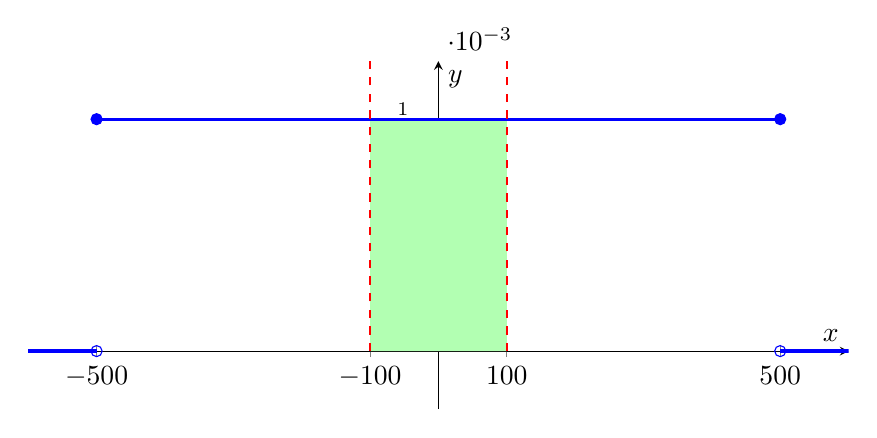
\begin{tikzpicture}
                \begin{axis}[
                axis lines=middle,
                xlabel={$x$},
                ylabel={$y$},
                xmin=-600, xmax=600,
                ymin=-0.0005, ymax=0.0025,
                xtick={-500,-100,0,100,500},
                xticklabels={$-500$,$-100$,$0$,$100$,$500$},
                ytick={0,0.002},
                yticklabels={$0$,$\frac{1}{500}$},
                width=12cm,
                height=6cm
                ]
                % Shaded area from -100 to 100 (the integral region)
                \addplot[fill=green!30, draw=none] coordinates {(-100,0) (-100,0.002) (100,0.002) (100,0)} \closedcycle;
                
                % The function g_500(x)
                \addplot[domain=-500:500, samples=2, very thick, blue] {0.002};
                \addplot[domain=-600:-500, samples=2, very thick, blue] {0};
                \addplot[domain=500:600, samples=2, very thick, blue] {0};
                
                % Mark the endpoints of g_500
                \addplot[only marks, mark=*, mark size=2pt, blue] coordinates {(-500,0.002) (500,0.002)};
                \addplot[only marks, mark=o, mark size=2pt, blue] coordinates {(-500,0) (500,0)};
                
                % Mark the integration bounds
                \addplot[dashed, thick, red] coordinates {(-100,0) (-100,0.0025)};
                \addplot[dashed, thick, red] coordinates {(100,0) (100,0.0025)};
                \end{axis}
            \end{tikzpicture}
            \end{center}
        
        Which has an area far less than $2$.

        Okay, so let's look at one last picture, and generalize our integral from that.

        \begin{center}
        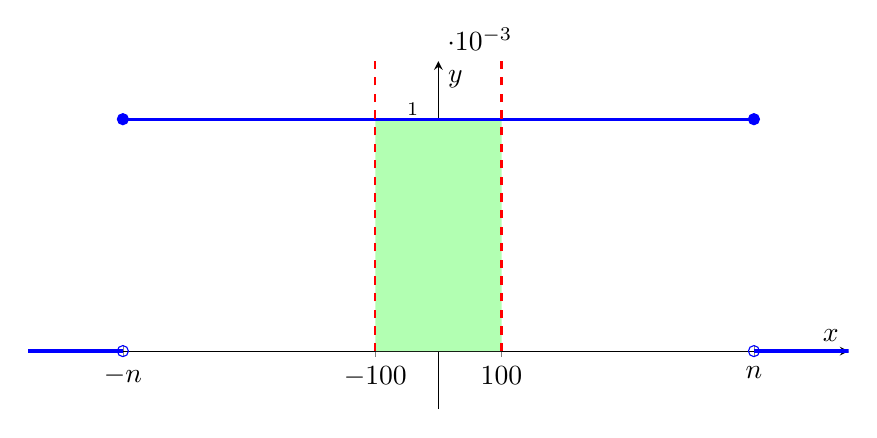
\begin{tikzpicture}
            \begin{axis}[
            axis lines=middle,
            xlabel={$x$},
            ylabel={$y$},
            xmin=-1.3, xmax=1.3,
            ymin=-0.0005, ymax=0.0025,
            xtick={-1,-0.2,0,0.2,1},
            xticklabels={$-n$,$-100$,$0$,$100$,$n$},
            ytick={0,0.002},
            yticklabels={$0$,$\frac{1}{n}$},
            width=12cm,
            height=6cm
            ]
            % Shaded area from -100 to 100 (the integral region)
            \addplot[fill=green!30, draw=none] coordinates {(-0.2,0) (-0.2,0.002) (0.2,0.002) (0.2,0)} \closedcycle;
            
            % The function g_n(x)
            \addplot[domain=-1:1, samples=2, very thick, blue] {0.002};
            \addplot[domain=-1.3:-1, samples=2, very thick, blue] {0};
            \addplot[domain=1:1.3, samples=2, very thick, blue] {0};
            
            % Mark the endpoints of g_n
            \addplot[only marks, mark=*, mark size=2pt, blue] coordinates {(-1,0.002) (1,0.002)};
            \addplot[only marks, mark=o, mark size=2pt, blue] coordinates {(-1,0) (1,0)};
            
            % Mark the integration bounds
            \addplot[dashed, thick, red] coordinates {(-0.2,0) (-0.2,0.0025)};
            \addplot[dashed, thick, red] coordinates {(0.2,0) (0.2,0.0025)};
            \end{axis}
        \end{tikzpicture}
        \end{center}

    
        Okay! We've got what we need!

        Using a super simple area of a rectangle thing, we have:

        Area = base $\cdot$ height.

        So, when $n > 100$, the height is $\frac{1}{n}$, and the base is $|100- (-100)| = 200$.

        \[ I_n = \begin{cases}
            2, & n \leq 100 \\
            \frac{200}{n}, & n > 100
        \end{cases} \]

    \end{proof}
\end{enumerate}